% coding:utf-8

%FOSAET, a LaTeX-Code for a electrical summary of basic electronics
%Copyright (C) 2013, Daniel Winz, Ervin Mazlagic

%This program is free software; you can redistribute it and/or
%modify it under the terms of the GNU General Public License
%as published by the Free Software Foundation; either version 2
%of the License, or (at your option) any later version.

%This program is distributed in the hope that it will be useful,
%but WITHOUT ANY WARRANTY; without even the implied warranty of
%MERCHANTABILITY or FITNESS FOR A PARTICULAR PURPOSE.  See the
%GNU General Public License for more details.
%----------------------------------------

\section{Logische Verknüpfungen}

\subsection{NOT}
\begin{figure}[h!]
  \begin{subfigure}{0.3\textwidth}
    \[ X = \overline{A} \]
  \end{subfigure}
  \begin{subfigure}{0.15\textwidth}
    \begin{tikzpicture}[circuit logic IEC]
      \node [not gate] (g) {};
      \draw (g.input) -- ++(left:3mm);
      \draw (g.output) -- ++(right:3mm);
    \end{tikzpicture}
  \end{subfigure}
  \begin{subfigure}{0.3\textwidth}
    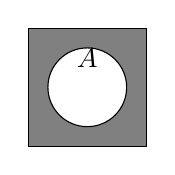
\begin{tikzpicture}[scale=0.5]
      \fill[gray] (-1.5,-1.5) rectangle (1.5,1.5);
      \draw (-1.5,-1.5) rectangle (1.5,1.5);
      \fill[white] (0,0) circle (1cm);
      \draw (0,0) circle (1cm);
      \draw (0,0.75) node {$A$};
    \end{tikzpicture}
  \end{subfigure}
  \begin{subfigure}{0.2\textwidth}
    \[ \begin{array}{c|c}
    A&X\\
    \hline
    0&1\\
    1&0
    \end{array} \]
  \end{subfigure}
\end{figure}

\subsection{OR}
\begin{figure}[h!]
  \begin{subfigure}{0.3\textwidth}
    \[ X = A \lor B \]
  \end{subfigure}
  \begin{subfigure}{0.15\textwidth}
    \begin{tikzpicture}[circuit logic IEC]
      \node [or gate] (g) {};
      \draw (g.input 1) -- ++(left:3mm);
      \draw (g.input 2) -- ++(left:3mm);
      \draw (g.output) -- ++(right:3mm);
    \end{tikzpicture}
  \end{subfigure}
  \begin{subfigure}{0.3\textwidth}
    \begin{venndiagram2sets}[tikzoptions={scale=0.5}]
      \fillA \fillB
    \end{venndiagram2sets}
  \end{subfigure}
  \begin{subfigure}{0.2\textwidth}
    \[ \begin{array}{cc|c}
    A&B&X\\
    \hline
    0&0&0\\
    0&1&1\\
    1&0&1\\
    1&1&1
    \end{array} \]
  \end{subfigure}
\end{figure}

\subsection{NOR}
\begin{figure}[h!]
  \begin{subfigure}{0.3\textwidth}
    \[ X = \overline{A \lor B} \]
  \end{subfigure}
  \begin{subfigure}{0.15\textwidth}
    \begin{tikzpicture}[circuit logic IEC]
      \node [nor gate] (g) {};
      \draw (g.input 1) -- ++(left:3mm);
      \draw (g.input 2) -- ++(left:3mm);
      \draw (g.output) -- ++(right:3mm);
    \end{tikzpicture}
  \end{subfigure}
  \begin{subfigure}{0.3\textwidth}
    \begin{venndiagram2sets}[tikzoptions={scale=0.5}]
      \fillNotAorB
    \end{venndiagram2sets}
  \end{subfigure}
  \begin{subfigure}{0.2\textwidth}
    \[ \begin{array}{cc|c}
    A&B&X\\
    \hline
    0&0&1\\
    0&1&0\\
    1&0&0\\
    1&1&0
    \end{array} \]
  \end{subfigure}
\end{figure}

\subsection{AND}
\begin{figure}[h!]
  \begin{subfigure}{0.3\textwidth}
    \[ X = A \land B \]
  \end{subfigure}
  \begin{subfigure}{0.15\textwidth}
    \begin{tikzpicture}[circuit logic IEC]
      \node [and gate] (g) {};
      \draw (g.input 1) -- ++(left:3mm);
      \draw (g.input 2) -- ++(left:3mm);
      \draw (g.output) -- ++(right:3mm);
    \end{tikzpicture}
  \end{subfigure}
  \begin{subfigure}{0.3\textwidth}
    \begin{venndiagram2sets}[tikzoptions={scale=0.5}]
      \fillACapB
    \end{venndiagram2sets}
  \end{subfigure}
  \begin{subfigure}{0.2\textwidth}
    \[ \begin{array}{cc|c}
    A&B&X\\
    \hline
    0&0&0\\
    0&1&0\\
    1&0&0\\
    1&1&1
    \end{array} \]
  \end{subfigure}
\end{figure}

\newpage

\subsection{NAND}
\begin{figure}[h!]
  \begin{subfigure}{0.3\textwidth}
    \[ X = \overline{A \land B} \]
  \end{subfigure}
  \begin{subfigure}{0.15\textwidth}
    \begin{tikzpicture}[circuit logic IEC]
      \node [nand gate] (g) {};
      \draw (g.input 1) -- ++(left:3mm);
      \draw (g.input 2) -- ++(left:3mm);
      \draw (g.output) -- ++(right:3mm);
    \end{tikzpicture}
  \end{subfigure}
  \begin{subfigure}{0.3\textwidth}
    \begin{venndiagram2sets}[tikzoptions={scale=0.5}]
      \fillNotAorNotB
    \end{venndiagram2sets}
  \end{subfigure}
  \begin{subfigure}{0.2\textwidth}
    \[ \begin{array}{cc|c}
    A&B&X\\
    \hline
    0&0&1\\
    0&1&1\\
    1&0&1\\
    1&1&0
    \end{array} \]
  \end{subfigure}
\end{figure}

\subsection{XOR}
\begin{figure}[h!]
  \begin{subfigure}{0.3\textwidth}
    \[ X = A \oplus B \]
  \end{subfigure}
  \begin{subfigure}{0.15\textwidth}
    \begin{tikzpicture}[circuit logic IEC]
      \node [xor gate] (g) {};
      \draw (g.input 1) -- ++(left:3mm);
      \draw (g.input 2) -- ++(left:3mm);
      \draw (g.output) -- ++(right:3mm);
    \end{tikzpicture}
  \end{subfigure}
  \begin{subfigure}{0.3\textwidth}
    \begin{venndiagram2sets}[tikzoptions={scale=0.5}]
      \fillANotB \fillBNotA
    \end{venndiagram2sets}
  \end{subfigure}
  \begin{subfigure}{0.2\textwidth}
    \[ \begin{array}{cc|c}
    A&B&X\\
    \hline
    0&0&0\\
    0&1&1\\
    1&0&1\\
    1&1&0
    \end{array} \]
  \end{subfigure}
\end{figure}

\subsection{XNOR}
\begin{figure}[h!]
  \begin{subfigure}{0.3\textwidth}
    \[ X = \overline{A \oplus B} \]
  \end{subfigure}
  \begin{subfigure}{0.15\textwidth}
    \begin{tikzpicture}[circuit logic IEC]
      \node [xnor gate] (g) {};
      \draw (g.input 1) -- ++(left:3mm);
      \draw (g.input 2) -- ++(left:3mm);
      \draw (g.output) -- ++(right:3mm);
    \end{tikzpicture}
  \end{subfigure}
  \begin{subfigure}{0.3\textwidth}
    \begin{venndiagram2sets}[tikzoptions={scale=0.5}]
      \fillNotAorB \fillACapB
    \end{venndiagram2sets}
  \end{subfigure}
  \begin{subfigure}{0.2\textwidth}
    \[ \begin{array}{cc|c}
    A&B&X\\
    \hline
    0&0&1\\
    0&1&0\\
    1&0&0\\
    1&1&1
    \end{array} \]
  \end{subfigure}
\end{figure}
